\newpage
\section{structure}

Luis Caires

Susan Eisenbach


\subsection{Interdisciplinary centres}

\begin{figure}[h]
\centering
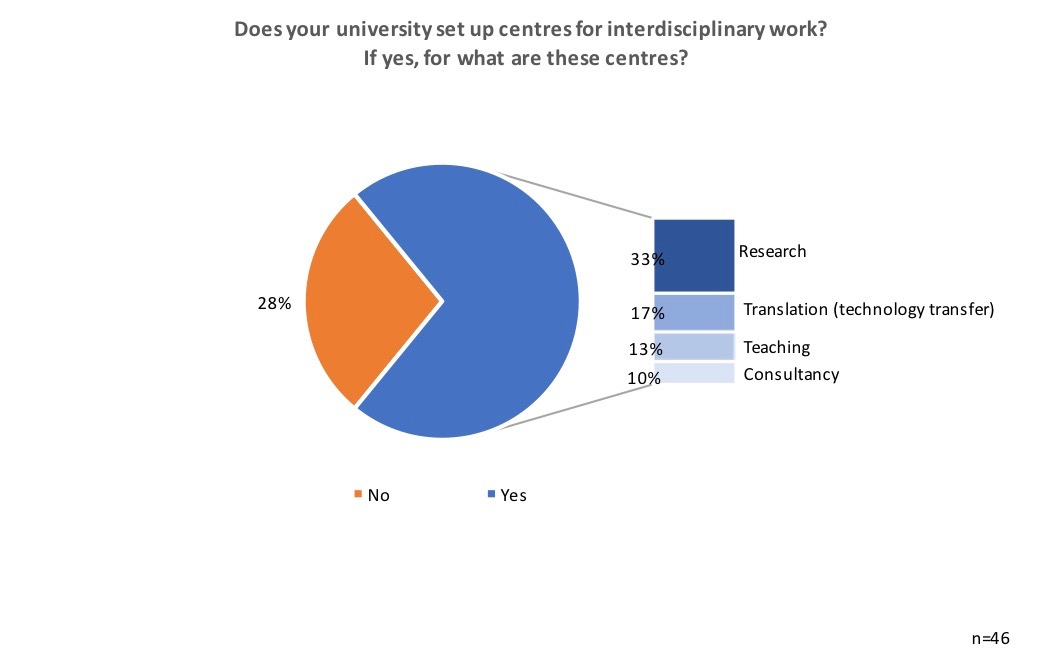
\includegraphics[width = \linewidth]{charts/5a.jpg}
\caption{What are the interdisciplinary centres?}
\label{sect5:centres}
\end{figure}

28\% of respondents say their university does not have real interdisciplinary centres (see Figure~\ref{sect5:centres}). Of those who commented on why the lack of centres only Aalto University actually replied that their management was averse to setting up additional administrative structures. The rest just said there were informal groupings, but nothing officially supported. 46\% of all of the interdisciplinary centres are set up primarily for research and only 18\% for teaching. The rest are primarily involved with industry.

There are a broad range of centres in the different universities -- clearly what expertise is in a university and what the structure of the different departments/schools/faculties impacts which centres are set up in addition to the existing primary structures. The most common centres mentioned with a significant Informatics component are in Computational Science (Delft, Aachen, Southern Denmark, Catalunya, Aalborg), Data Science (Imperial College, P Milano, Lugano, Paderborn, Tilburg),  Life Science (Babes-Bolyai,  Edinburgh, Humboldt, Lugano, Masaryk, Tarfu), Digital Society (ETH, Zurich, Sofia), Energy (Delft, ETH, TU Wien), and Security(Edinburgh, Imperial, P Milano).   There were two universities with the following centres: Biomedical Engineering (EPFL, Catalunya), Environment/Climate (ETH, Humboldt),  Medical Imaging (ETH, Imperial), and  Complex Systems (TU Wien, Utrecht). There are a wide range of centres which only mentioned at one university: Health (Delft),  FinTech (Zurich), Digital Humanities (E\" otv\"os Lor\'and), Robotic Surgery (Imperial ), Cognitive Ageing (Edinburgh), Bioinformatics (P Milano), and Geoinformatics (P Milano), 
 


\subsection{Purpose of interdisiciplinary centres}

\begin{figure}[h]
\centering
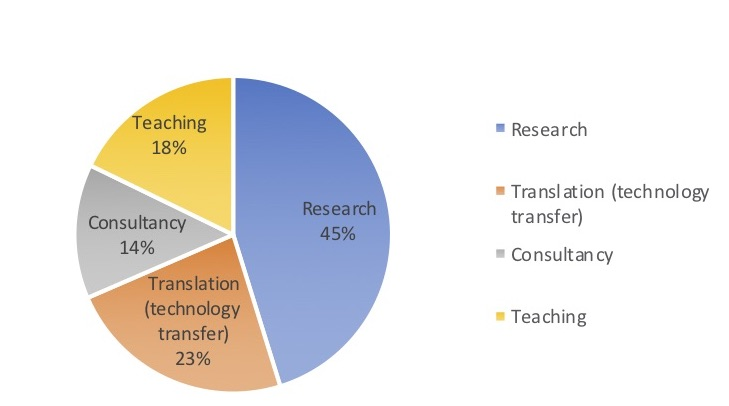
\includegraphics[width = \linewidth]{charts/5b.jpg}
\caption{Why were the centres created?}
\label{sect5:reasons}
\end{figure}

45\% of all of the interdisciplinary centres are set up primarily for research and only 18\% for teaching. The rest are primarily involved with industry collaboration or consultancy.

\subsection{ Ownership of interdisciplinary centres}

Of the 36 respondents, 21 (or 58\%) are independent entities within their university, 12 (or 1/3) are co-owned by the departments that are involved and the rest have a single department that owns them. It is surprising that so many are separate entities as this means if they are not self-funding

\begin{figure}[h]
\centering
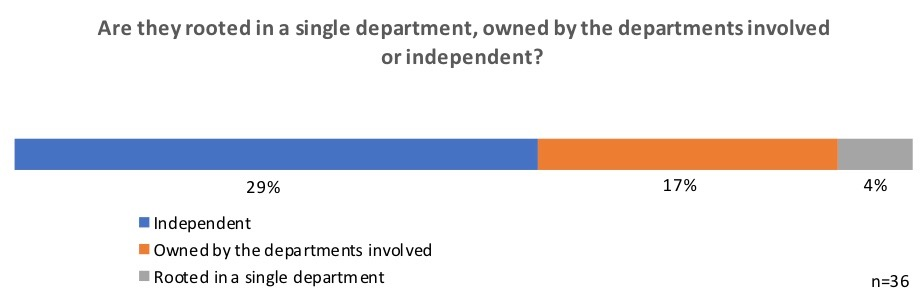
\includegraphics[width = \linewidth]{charts/5c.jpg}
\caption{Which entity control the interdisciplinary centres?}
\label{sect5:owners}
\end{figure}

\subsection{ Location of interdisciplinary centres}

\begin{figure}[h]
\centering
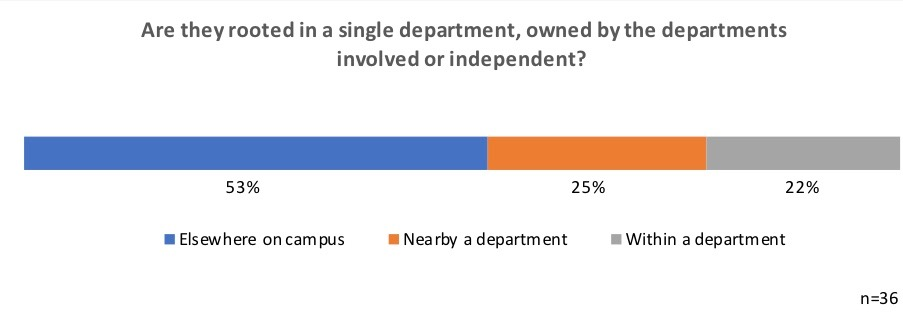
\includegraphics[width = \linewidth]{charts/5d.jpg}
\caption{ Where are the centres located?}
\label{sect5:locations}
\end{figure}

\subsection{Funding of interdisciplinary centres}

\begin{figure}[h]
\centering
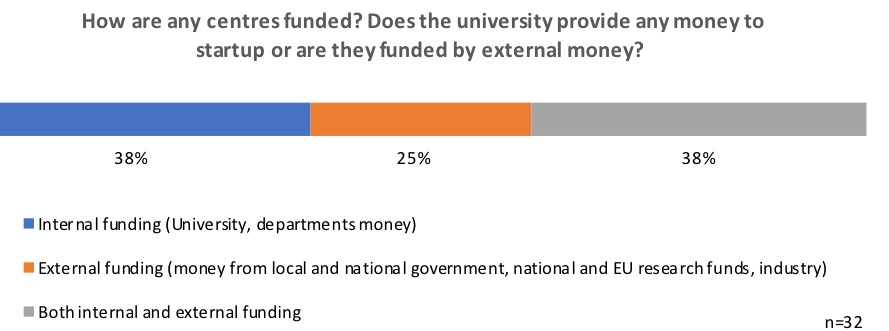
\includegraphics[width = \linewidth]{charts/5e.jpg}
\caption{Who funds interdisciplinary centres?}
\label{sect5:funding}
\end{figure}

\subsection{Planning for changing interdisciplinary centres}

\begin{figure}[h]
\centering
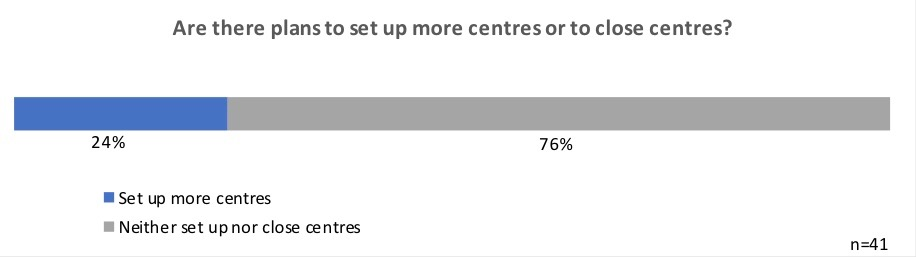
\includegraphics[width = \linewidth]{charts/5f.jpg}
\caption{Are there changes planned for setting up or closing centres?}
\label{sect5:changes}
\end{figure}

\subsection{Drivers for new activities}

\begin{figure}[h]
\centering
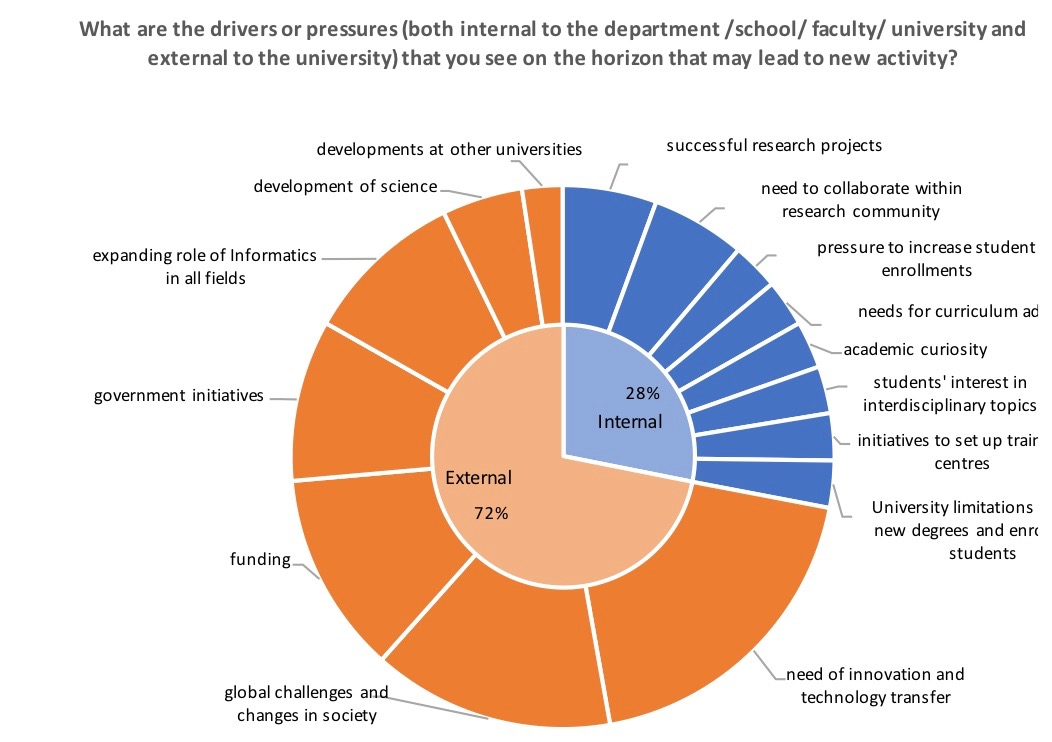
\includegraphics[width = \linewidth]{charts/5g.jpg}
\caption{What are the drivers for new centres?}
\label{sect3:drivers}
\end{figure}

\subsection{Support for interdisciplinary work}

\begin{figure}[h]
\centering
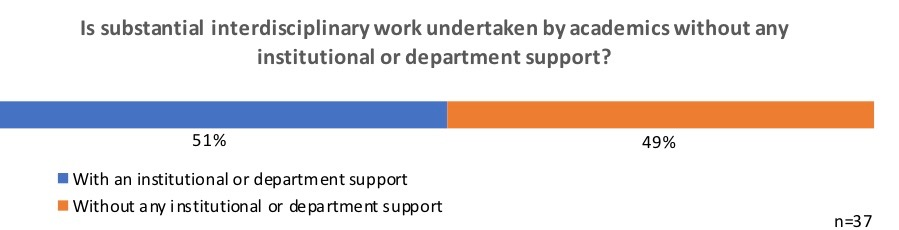
\includegraphics[width = \linewidth]{charts/5h.jpg}
\caption{How much support is provided for interdisciplinary work?}
\label{sect5:support}
\end{figure}

\subsection{Strategic vision }
\begin{figure}[h]
\centering
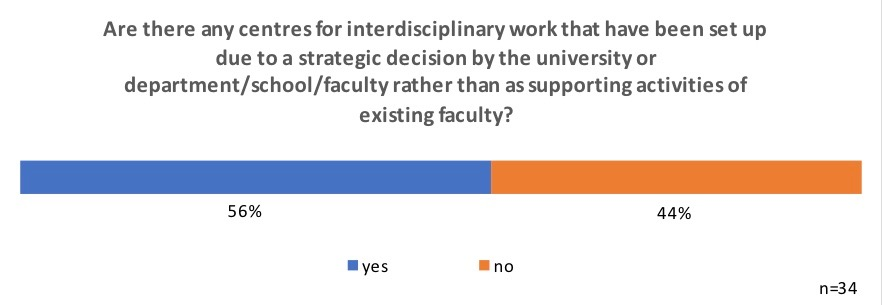
\includegraphics[width = \linewidth]{charts/5i.jpg}
\caption{Interdisciplinary hirings}
\label{sect5:strategy}
\end{figure}

\subsection{Official strategic vision}
\begin{figure}[h]
\centering
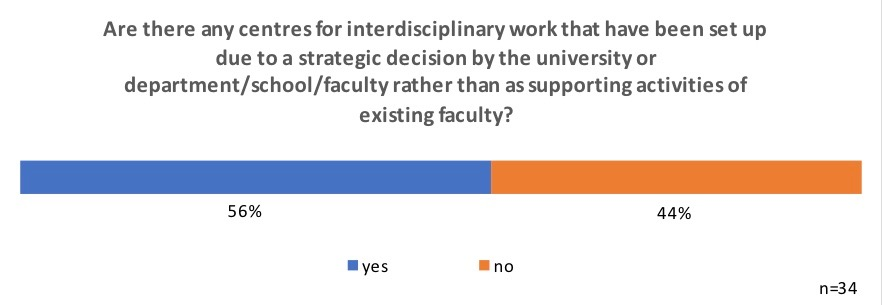
\includegraphics[width = \linewidth]{charts/5i.jpg}
\caption{Is there an official strategy to widen the role of Informatics?}
\label{sect5:official}
\end{figure}

\subsection{Final thoughts}





